\documentclass[text05.tex]{subfiles}
\begin{document}
\subsubsection{照度センサー}\label{light}
\begin{table}[H]
  \begin{widerrows}
    \begin{tabular}{|p{\colF}|p{\colG}|}	\hline
    \ruby{名称}{めい|しょう} & 照度センサー（しょうどせんさー）\\ \hline
    \ruby{接続箇所}{せつ|ぞく|か|しょ} & アナログコネクタ (3pin)\\ \hline
    \ruby{機能概要}{き|のう|がい|よう} & 周辺の明るさの\ruby{測定}{そく|てい}\\ \hline
    \end{tabular}
  \end{widerrows} 
\end{table}

\begin{table}[H]
  \begin{widerrows}
    \begin{tabular}{|p{\colF}|p{\colG}|}	\hline
    サンプルコードの場所 & 05/anain.hsp\\ \hline
    raspiへの入力 & 明るさを表す0から1023の\ruby{値}{あたい}。明るいと\ruby{値}{あたい}が\ruby{減}{へ}り、暗いと\ruby{値}{あたい}が\ruby{増}{ふ}える。\\ \hline
    raspiへの入力方法 & val = \adcget(ピン番号, チャンネル番号)\\ \hline
    raspiからの出力 & なし\\ \hline
    raspiからの出力方法 & なし\\ \hline
    \end{tabular}
  \end{widerrows} 
\end{table}

\begin{table}[H]
  \begin{widerrows}
    \begin{tabular}{|p{\colF}|p{\colG}|} \hline
    使い道 & 照度\ruby{計測}{けい|そく}、カメラの\ruby{露出}{ろ|しゅつ}調節\ruby{機能}{き|のう}に。\\ \hline
    \ruby{注意事項}{ちゅう|い|じ|こう} & 材料の\ruby{硫化}{りゅう|か}カドミウム(CdS)は人体に有害なため、\ruby{割}{わ}れたセンサーを\ruby{素手}{す|で}で\ruby{触}{さわ}らないこと。\\ \hline
    \ruby{補足}{ほ|そく} & なし\\ \hline
    \end{tabular}
  \end{widerrows} 
\end{table}

\begin{figure}[H]
  \begin{widerrows}
    \begin{tabular}{|p{\colH}|p{\colI}|p{\colH}|p{\colI}|} \hline
    外観 & 
    \begin{minipage}[t]{\linewidth}
      \smallskip
        \centering
        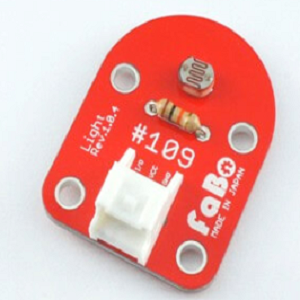
\includegraphics[width=0.5\linewidth]{../../asset/image/text05-img024.png}
        \caption{照度センサー}
        \smallskip
      \end{minipage} &
      回路記号 & 
      \begin{minipage}[t]{\linewidth}
      \smallskip
        \centering
        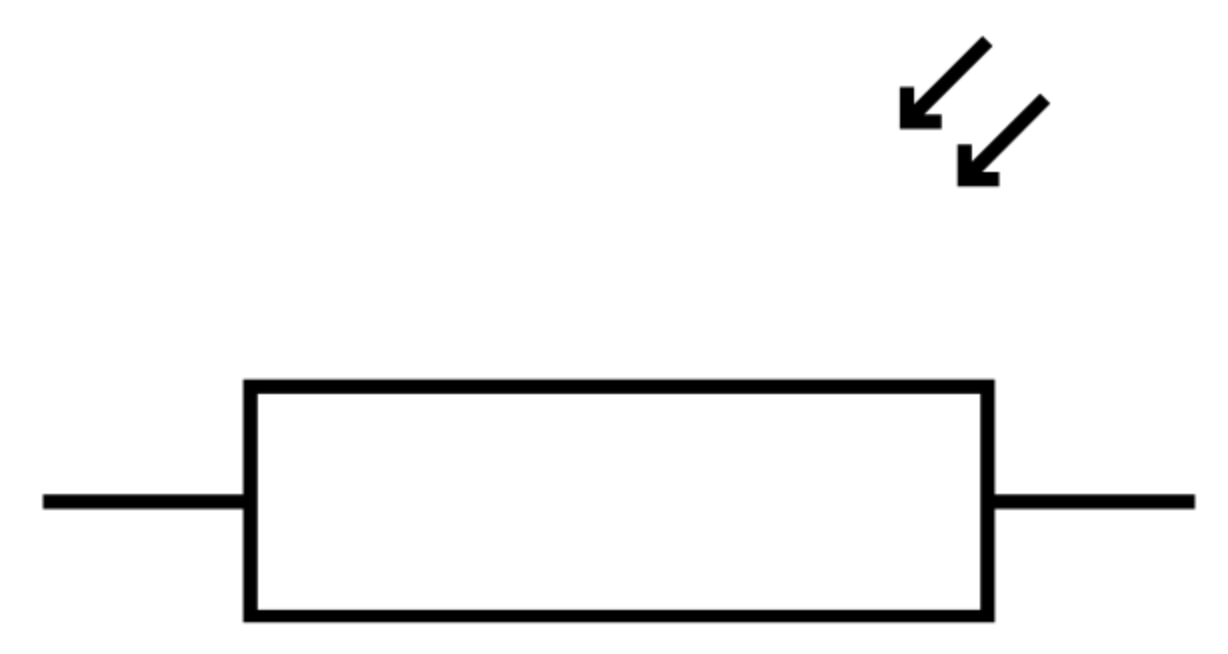
\includegraphics[width=0.5\linewidth]{../../asset/image/text05-img053.png}
        \caption{照度センサーの回路図}
        \smallskip
      \end{minipage}\\ \hline
    \end{tabular}
  \end{widerrows} 
\end{figure}
\end{document}
